\chapter{Задача оптимального экономического роста}\label{chap2}


В данной главе исследуется задача оптимального экономического роста в неоклассической модели с логарифмической функцией мгновенной полезности.  Эти задачи представляют интерес в связи с тем, что они могут выбираться в качестве прогнозирующих задач оптимального управления при применении теории главы 1 для решения задачи роста.

%%%%%%%%%%%%%%%%%%%%%%%%%%%%%%%%%%%%%%%%%%%%%%%%%%%%%%%%%%%%%%%%%%%%%%%%%%%%%%%%
\section{Неоклассическая модель экономического роста}\label{2sec:problem-formulation}
%%%%%%%%%%%%%%%%%%%%%%%%%%%%%%%%%%%%%%%%%%%%%%%%%%%%%%%%%%%%%%%%%%%%%%%%%%%%%%%%
Неоклассическая модель оптимального экономического роста описывает замкнутую агрегированную экономику, производящую в каждый момент времени $ t \ge 0$ 
единственный однородный продукт (капитал) со скоростью $ Y(t)>0 $. В каждый момент времени $ t $ величина $ Y (t) $ является функцией текущих значений капитала $ K(t) > 0 $ и трудовых ресурсов $ L(t) > 0 $; трудовые ресурсы также предполагаются однородными. Таким образом, \\
\begin{equation}
Y (t)=F(K(t),L(t)) \text{ для любого } t \ge 0. 
\end{equation}
Функция $ F $ обычно называется производственной функцией. Относительно производственной функции $ F $ предполагается, что она определена и непрерывна на положительном квадранте \\
\begin{center}
	$G ={(K,L) \in \mathbb{R}^2: K>0, L >0},$
\end{center}
дважды непрерывно дифференцируема и удовлетворяет следующим неоклассическим условиям 
для всех K>0, L>0: \\
\begin{equation}
\dfrac{\partial F (K, L)}{\partial K} < 0 \hspace{2cm}  \dfrac{\partial^2 F (K, L)}{\partial K^2} < 0
\end{equation}
\begin{equation}
\dfrac{\partial F (K, L)}{\partial L} < 0 \hspace{2cm}  \dfrac{\partial^2 F (K, L)}{\partial L^2} < 0
\end{equation}\\
\begin{equation}
\underset{K \rightarrow +0}{lim} \dfrac{\partial F (K, L)}{\partial K} = \infty \hspace{1cm} \underset{K \rightarrow \infty}{lim} \dfrac{\partial^2 F (K, L)}{\partial K^2} = 0
\end{equation}
\begin{equation}
\underset{L \rightarrow +0}{lim} \dfrac{\partial F (K, L)}{\partial L} = \infty \hspace{1cm} \underset{L \rightarrow \infty}{lim} \dfrac{\partial^2 F (K, L)}{\partial L^2} = 0
\end{equation}
Наконец, предполагается, что $ F $ положительно однородна первой степени, т.е. \\
\begin{equation}
F(\lambda K,\lambda L)=\lambda F(K,L) \hspace{1cm} \text{для любых} \lambda>0, K > 0, L > 0
\end{equation}
Последнее условие означает, что объем производства в каждую единицу времени прямо пропорционален величинам имеющихся в эту единицу времени производственных факторов. В качестве производственной функции $ F $ может фигурировать, например, стандартная функция Кобба-Дугласа вида \\
\begin{center}
	$ F(K,L)=AK^{\alpha_1}L^{\alpha_2} $,
\end{center}
где $ A>0, \alpha_1 > 0, \alpha_2 > 0 $ и $ \alpha_1 + \alpha_2 =1 $ . \\
Заметим, что в силу равенства (2.6) не все условия в (2.2)---(2.5) независимы. В частности, второе условие в (2.3) следует из второго условия в (2.2) и (2.6).

В замкнутой экономике произведенный продукт либо инвестируется в основные производственные фонды (капитал), либо потребляется. Предположим, что в каждый момент времени $ t \ge 0 $ минимально возможная часть потребляемого продукта есть $  \varepsilon Y (t) > 0 $, где $ 0 <\varepsilon<1 $ - некоторая постоянная, а доля продукта $ (1 - \varepsilon) Y (t) $ может быть распределена между производством и потреблением произвольным образом.

Пусть в момент времени $ t \ge 0 $ часть \\
\begin{equation}
I(t) = u(t)Y (t), 0 \ge u(t) \ge 1-\varepsilon, 
\end{equation}
произведенного продукта инвестируется в основные производственные фонды, а оставшаяся часть \\
\begin{equation}
C(t) = (1-u(t))Y (t) 
\end{equation}
потребляется. В дальнейшем величина $ u(t)\in[0,1-\varepsilon] $ будет трактоваться как значение управления в момент времени $ t $. 

В данной модели амортизации капитала не предполагается. Поэтому в силу равенства (2.7) динамика изменения капитала может быть описана при помощи следующего дифференциального уравнения: 
\begin{equation}
\dot{K}(t)=I(t)=u(t)Y (t). 
\end{equation}
Считаем, что в начальный момент времени $ K(0) = K_0 > 0.  $

Пусть трудовые ресурсы удовлетворяют условию экспоненциального роста, т.е. 
\begin{equation}
\dot{L}(t)=\mu L(t),
\end{equation}
где $ \mu>0 $ --- некоторая постоянная. Аналогично будем считать, что $ L(0) = L_0 > 0.  $\\
Пусть $  \rho>0 $ - параметр дисконтирования и в каждый момент времени $ t \ge 0 $ мгновенная полезность $ g(K(t),L(t),u(t)) $ текущего процесса управления есть логарифм полного потребления $ C(t) $, т.е. (см. (2.1), (2.8))
\begin{center}
	$ 	g(K(t),L(t),u(t)) = \ln C(t) = \ln (1-u(t))+\ln F(K(t),L(t)).  $
\end{center} 

\section{Задача оптимального управления для неоклассической модели экономики c логарифмической функцией мгновенной полезности}
Неоклассическая модель оптимального экономического роста (c логарифмической функцией мгновенной полезности) формулируется в виде следующей задачи оптимального управления $ (P_\varepsilon), 0 <\varepsilon<1 $: 
\begin{equation}
J(K,L,u)= \int_{0}^{\infty}
e^{-\rho t}[\ln(1-u(t))+\ln F(K(t),L(t))]dt \rightarrow \max.
\end{equation}
\begin{center}
	$ \dot{K}(t)=u(t)F(K(t),L(t)),\hspace{1cm} u(t)\in U_\varepsilon = [0 ,1-\varepsilon],  $\\
	$\dot{L}(t)=\mu L(t),$\\
	$ K(0) = K_0,L (0) = L_0, $
\end{center} 

При исследовании неоклассической задачи оптимального экономического роста обычно, используя условие однородности (2.6), понижают размерность системы и переходят к вспомогательной фазовой переменной $ x = K/L $ (величине капитала, приходящегося на единицу рабочей силы) и однофакторной производственной функции $ f $ вида $ f(x)=F(x,1) $, x>0. В этом случае в силу условий (2.1) и (2.6) для любого $ t \ge 0 $ 
\begin{center}
	$ \dfrac{Y(t)}{L(t)}=
	\dfrac{1}{L(t)}F(K(t),L(t)) = F \left(\dfrac{K(t)}{L(t)},1\right) = f(x(t)).
	$
\end{center} 
Функция $ f $ определена и непрерывна на $\tilde{G} = (0 ,\infty$). В силу условий (2.2) для всех $ x>0  $
\begin{equation}
\frac{d}{dx}f(x) > 0, \hspace{1cm} \frac{d^2}{d^2x}f(x) < 0 
\end{equation}
и вследствие (2.2)-(2.6)
\begin{equation}
\underset{x \rightarrow +0}{lim} f(x) = 0 \hspace{0.7cm} \underset{x \rightarrow \infty}{lim} f(x) = \infty \hspace{0.7cm} \underset{x \rightarrow +0}{lim} \frac{d}{dx} f(x) = \infty \hspace{0.7cm} \underset{x \rightarrow \infty}{lim} \frac{d}{dx} f(x) = 0
\end{equation}
Для переменной $ x(t)=K(t)/L(t) $ в силу равенств (2.9) и (2.10) имеем
\begin{center}
	$ \dot{x}(t)=\dfrac{d}{dt}\dfrac{K(t)}{L(t)} = \dot{K}(t)\dfrac{1}{L(t)} - \dfrac{K(t)}{L^2(t)}\dot{L}(t) = u(t)\dfrac{Y(t)}{L(t)} - \mu \dfrac{K(t)}{L(t)} $
\end{center}
откуда в силу определения переменной $ x $ и условий (2.1) и (2.6) вытекает равенство
\begin{center}
	$\dot{x}(t)=u(t)f(x(t))-\mu x(t).  $
\end{center}
Величина мгновенного потребления на единицу трудовых ресурсов в момент времени $ t \ge 0 $ есть $ c(t)=C(t)/L(t) $. Согласно (2.1) и (2.8) получаем 
\begin{center}
	$ c(t) = (1-u(t))\dfrac{Y(t)}{L(t)} = (1-u(t))f(x(t)).  $
\end{center}

Заметим, что в силу равенства (2.10) трудовые ресурсы $ L $ в рассматриваемой модели подчиняются заранее заданной динамике. Поэтому максимизация интегрального функционала (2.11) эквивалентна задаче максимизации функционала
\begin{center}
	$ J(x,u)= \int_{0}^{\infty}
	e^{-\rho t} \ln c(t)dt =
	\int_{0}^{\infty}
	e^{-\rho t}[\ln(1-u(t))+\ln f(x(t))]dt,  $
\end{center}
характеризующего агрегированную удельную скорость роста потребления на единицу рабочей силы.

Пусть в задаче $ (P_\varepsilon) $ существует оптимальное допустимое управление $ u_* $. Тогда пусть $ (K_*,L_*) $ --- соответствующая управлению $ u_* $ допустимая траектория.
В силу неоклассических условий (2.2)---(2.5) и положительности производственной функции $ F $ имеем 
\begin{center}
	$ \dfrac{\partial \ln F(R, L)}{\partial K} = \dfrac{1}{F(K, L)}\dfrac{\partial F(R, L)}{\partial K} > 0$  для любых  $K>0, L > 0 $\\
	$ \dfrac{\partial \ln F(R, L)}{\partial L} = \dfrac{1}{F(K, L)}\dfrac{\partial F(R, L)}{\partial L} > 0$  для любых  $K>0, L > 0 $
\end{center}
Для вектора $ u_0 =1-\varepsilon \in U_\varepsilon $ правая часть управляемой системы в начальной точке $ (K_0,L_0) $ положительна. В таком случае, для задачи $ (P_\varepsilon) $ выполняется теорема 10.1 из публикации Асеева и Кряжимского [3]. К тому же, можно утверждать, что оптимальное управление $ u_* $ таково, что для некоторого положительного числа $ \theta $ начиная с некоторого момента времени $ \tau \ge 0 $ выполняется неравенство $ u_* (t) \ge \theta$, то для данного управления $ u_* $ выполняются следующие условия 
\begin{center}
	$ x_*(t) \ge 0 $ для любого $ t \ge \tau $\\
	$ \dfrac{\partial f(x_*(t),u_*(t))}{\partial x} - \theta  I \ge 0 $ при почти всех $ t \ge \tau ,$
\end{center}
где $ I^- (n\times n) $-единичная диагональная матрица. Тогда сопряженная переменная $ \psi  $, соответствующая оптимальной паре $ (x_*,u_*) $ удовлетворяет условию трансверсальности. Следовательно, в этом случае соответствующая оптимальной тройке $ (K_*,L_*,u_*) $ в силу принципа максимума в нормальной форме  сопряженная переменная $ \psi =( \psi^1,\psi^2) $ удовлетворяет условию трансверсальности. 

Используя теорему 10.1, о которой шла речь выше, в публикации [3] выводится видоизмененный принцип максимума Понтрягина. Он даст нам соотношения, которых будет вполне достаточно для однозначной характеризации всех оптимальных режимов в задаче $ (P_\varepsilon) $. Мы рассмотрим задачу $ (P_\varepsilon) $ при произвольном малом параметре $ \varepsilon>0 $. При этом будет показано, что для любого начального состояния $ (K_0,L_0) \in G $ в случае, когда параметр $ \varepsilon $ достаточно мал, значение этого параметра $ \varepsilon $ никакого влияния на оптимальную тройку $ (K_*,L_*,u_*) $ не оказывает.

Таким образом, в терминах фазовой переменной x задача оптимального управления ($P_\varepsilon$), $ 0 <\varepsilon<1 $, переписывается в виде следующей задачи ($\tilde{P}_\varepsilon$):
\begin{center}
	$ J(x,u) = \int_{0}^{\infty}
	e^{-\rho t}[\ln(1-u(t))+\ln f(x(t))]dt \rightarrow \max.$\\
	$ \dot{x}(t) = u(t) f(x(t))-\mu x(t),u (t)\in U_\varepsilon = [0 ,1-\varepsilon], $\\
\end{center}
\begin{equation}
x(0) = x_0,
\end{equation}

Здесь $ x_0\in \tilde{G} = {x \in \mathbb{R}^1: x>0} $ и $ f(x)=F(x,1) $ для любого $ x \in \tilde{G}. $ Остальные данные в задаче $ (\tilde{P}_\varepsilon) $ те же самые, что и в задаче $ ( P_\varepsilon) $.\\
%%%%%%%%%%%%%%%%%%%%%%%%%%%%%%%%%%%%%%%%%%%%%%%%%%%%%%%%%%%%%%%%%%%%%%%%%%%%%%%%
\section{Построение магистралей}
Магистралью мы называем равновесное положение экономической системы. Для её в данной задаче мы должны построить гамильтонову систему принципа максимума для $(\tilde{P}_\varepsilon)$. 

В силу теоремы 15.2 [3], предлагающей нам еще один вариант принципа максимума Понтрягина в терминах сопряженной переменной $ p $, текущей функции Гамильтона–
Понтрягина $ \cal{M} $ и текущего гамильтониана $ M $ для любого $ t \ge 0 $ имеем $ p(t) > 0 $. Так как все допустимые траектории $ x $
управляемой системы $ \dot{x}(t) = u(t) f(x(t))-\mu x(t),u (t)\in U_\varepsilon = [0 ,1-\varepsilon], $ положительные, то любая пара $ (x_*,p) $, где $ x_* $ — оптимальная траектория в задаче $ (\tilde{P}_\varepsilon) $, а $ p $ — соответствующая ей текущая сопряженная переменная, при
всех значениях $ t \ge 0 $ принимает значения в положительном квадранте
\begin{center}
	Г$  = {(x,p) \in \mathbb{R}^2 : x > 0, p > 0.} $
\end{center}

Построим гамильтонову систему принципа максимума для задачи $(\tilde{P}_\varepsilon)$ в открытом множестве Г

Разрешая условие максимума относительно управления $ u $ в множестве Г, получаем, что максимум в фунции Гамильтона-Понтрягина достигается в точке
\begin{equation*}
u(x,p)= 
\begin{cases}
0, если 0 < p < \dfrac{1}{f(x)},\\
1 - \dfrac{1}{f(x)p}, если \dfrac{1}{f(x)} \le p \le \dfrac{1}{\varepsilon f(x)},\\
1 - \varepsilon, если p > \dfrac{1}{\varepsilon f(x)},
\end{cases}
\end{equation*}
и всюду в множестве Г имеем
\begin{center}
	$ M(x,p)=(u(x,p)f(x) - \mu x) p + \ln(1 - u(x,p)) + \ln f(x). $
\end{center}

В соответствии с вышеуказанным условаием определим множества Г$_1$, Г$_2$ и Г$_3$:
\begin{center}
Г$_1 = {(x,p)\in} $Г$: 0 < p < \dfrac{1}{f(x)} $, Г$_2 = {(x,p)\in} $Г$: \dfrac{1}{f(x)} \le p \ge \dfrac{1}{\varepsilon f(x)} $,\\
Г$_3 = {(x,p)\in} $Г$: p > \dfrac{1}{\varepsilon f(x)} $
\end{center}

Логично, что Г = Г$_1 \cup $Г$_2 \cup $Г$_3$

В множестве Г$_1$ гамильтонова система принципа максимума имеет вид
\begin{equation}
\dot{x} = -\mu x(t),\\
\dot{p}(t)=(\rho + \mu)p(t) - \dfrac{1}{f(x(t))} \dfrac{d}{dx}f(x(t)).
\end{equation}
Таким образом, в множестве Г$_1$ положений равновесия у гамильтоновой системыпринципа
максимума нет. Все ее траектории имеют в этом множестве экспоненциально убывающую
координату $ x $.
Определим функцию $ y_1 : (0,\infty) \rightarrow \mathbb{R}^1  $ равенством
\begin{center}
$ y_1(x)=\dfrac{1}{(\rho + \mu)f(x)} \dfrac{d}{dx}f(x) $  для любого  $ x > 0 $.
\end{center}
В силу неоклассических условий функция $ y_1 $ монотонно убывает,
\begin{center}
$ y_1(x) \rightarrow \infty $ при $ x \rightarrow 0  $и $ y_1(x) \rightarrow 0 $ при $ x \rightarrow \infty $,
\end{center}
а равенство $ y1(x)=1/f(x) $ выполняется в единственной точке $ \hat{x} $, являющейся корнем уравнения
\begin{equation}
\dfrac{d}{dx}f(x) = \rho + \mu
\end{equation}

Определив кривые $ V^0_{12}, V^0_{21}, V^0_{22}, V^0_{31}, V^0_{32} $, а так же множества, на которые они разбивают Г$_1$, Г$_2$ и Г$_3$, мы можем построить характер поведения траекторий гамильтоновой системы принципа максимума Понтрягина для задачи  $ (\tilde{P}_\varepsilon) $ [3]:
\begin{center}
	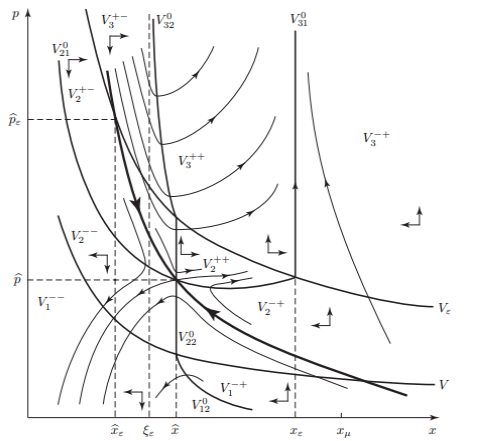
\includegraphics[width=10cm]{dugi}
\end{center}

Точка $ (\hat{x}, \hat{p}) $ будет считаться равновесной в данной системе и пренадлежать множеству Г$_2$, т.к. все траектории Г$_1$ имеют экспоненциальную убывающую координату $ x $ (см. расчеты выше), а во множестве Г$_3$ прямая $  V^0_{31} $ и кривая $ V^0_{32} $ не пересекаются (см. рис.).

Соответственно, используя (2.16) для рассчета $ \hat{x} $ и формулу  $ \hat{p} = \dfrac{1}{f(\hat{x}) - \mu\hat{x}} $ мы получаем нашу точку $ (\hat{x}, \hat{p}) $.
Чтобы перейти к определенным в предыдущем пункте  $ (x_*, u_*) $ воспользуемся следующими формулами:
\begin{center}
	$ x_*(t) \equiv x, u_*(t) =1 - \dfrac{1}{f(\hat{x})\hat{p}}$
\end{center}
К ним переходим в силу следствия 15.2 [3], по которому положение равновесия $ (\hat{x}, \hat{p}) $  соответствует оптимальной стационарной траектории с начальным условием $ x_0 = \hat{x} $ для управляемой системы $ \dot{x}(t) = u(t) f(x(t))-\mu x(t),u (t)\in U_\varepsilon = [0 ,1-\varepsilon] $ из задачи $(\tilde{P}_\varepsilon)$.
